% PROVISIONAL WORKING STYLE: IASEAI'27 has not yet published its detailed paper
% formatting guide. This AAAI-2027-style source is a working layout only; re-check
% the official IASEAI'27 instructions before submission and do not modify aaai2027.sty.
\documentclass[letterpaper]{article}
\usepackage[submission]{aaai2027}
\usepackage[hyphens]{url}
\usepackage{graphicx}
\urlstyle{rm}
\def\UrlFont{\rm}
\usepackage{natbib}
\usepackage{caption}
\frenchspacing
\usepackage{booktabs}
\usepackage{amsmath,amssymb}
\usepackage{tikz}
\usetikzlibrary{positioning,arrows.meta,calc}
\usepackage{xcolor}
\pdfinfo{/TemplateVersion (2027.1)}
\setcounter{secnumdepth}{1}

\title{The Imperfective Uncertainty in Large Language Models}
\author{Anonymous Submission}
\affiliations{}

\begin{document}
\maketitle

\begin{abstract}
Large language models (LLMs) can mistake an action in progress for an action completed, a failure isolated by the ImperfectiveNLI diagnostic benchmark. We study a complementary question: \emph{what uncertainty do models express when completion is not semantically licensed, and is that uncertainty useful for risk control?} The imperfective paradox offers an unusually clean test because an ambiguous telic progressive leaves the real-world endpoint under-specified while the corresponding natural-language-inference (NLI) target is determinately \textsc{Unknown}. We therefore distinguish \emph{semantic uncertainty} about the event from \emph{predictive uncertainty} about the model's inference. Across five cross-family gateway-routed LLM endpoints, we evaluate structured verbal label probabilities, repeated-sampling disagreement, calibration, error ranking, prompt sensitivity, paired context updates, and selective rechecking on ImperfectiveNLI. We preserve the benchmark's group accuracy, Teleological Bias Rate, and Aspectual Awareness Gap while adding proper scoring rules, uncertainty-specific diagnostics, verb-cluster bootstrap intervals, and risk--coverage analysis. We predeclare a neutral primary prompt so that the main experiment measures model behavior rather than explicit instruction in aspectual semantics; strict-logic and definition-aware prompts are robustness conditions only. All numerical results and empirical conclusions remain \textbf{TBD} until frozen API artifacts pass an automated manifest-aware audit. The study is designed to test not merely whether LLMs make aspectual errors, but whether their uncertainty makes those errors detectable and controllable without inducing indiscriminate skepticism toward valid atelic entailments.
\end{abstract}

\section{Introduction}
LLMs increasingly serve as components of agents, monitors, copilots, and decision-support systems that must infer whether described actions have actually occurred. A deceptively small linguistic distinction can matter operationally. ``The technician was repairing the brake'' describes a process in progress; ``the technician repaired the brake'' conventionally presents a completed result. A system that collapses these states can turn an unfinished action into an assumed fact, potentially propagating an unsupported success condition into later reasoning.

The \emph{Imperfective Paradox} formalizes this contrast. Progressive activities such as \emph{running} license occurrence of the activity, whereas progressive accomplishments such as \emph{building a house} do not entail attainment of their inherent endpoint \citep{vendler-1957-verbs,dowty-1979-word,comrie-1976-aspect}. Ma and Miyao introduced ImperfectiveNLI and reported a strong \emph{Teleological Bias}: several open-weight LLMs infer completion for goal-directed events, sometimes even when context explicitly cancels the endpoint \citep{ma-miyao-2026-imperfective}. They further showed that stronger aspect-oriented prompting can suppress completion errors while over-correcting on atelic activities, creating a reliability trade-off.

That benchmark exposes a second problem that is not reducible to accuracy: \textbf{imperfective uncertainty}. In its critical ambiguous-accomplishment condition (Group C), the described world outcome is semantically unresolved, but the classification target is not: the NLI relation is \textsc{Unknown}. Thus a competent reasoner should be \emph{confidently uncertain about the event}. High probability on \textsc{Unknown} reflects recognition of under-specification; high probability on \textsc{True} reflects teleological overconfidence; a nearly uniform distribution over \{True, False, Unknown\} reflects predictive confusion rather than semantic competence. Figure~\ref{fig:concept} makes this distinction explicit.

\begin{figure}[t]
\centering
\resizebox{\columnwidth}{!}{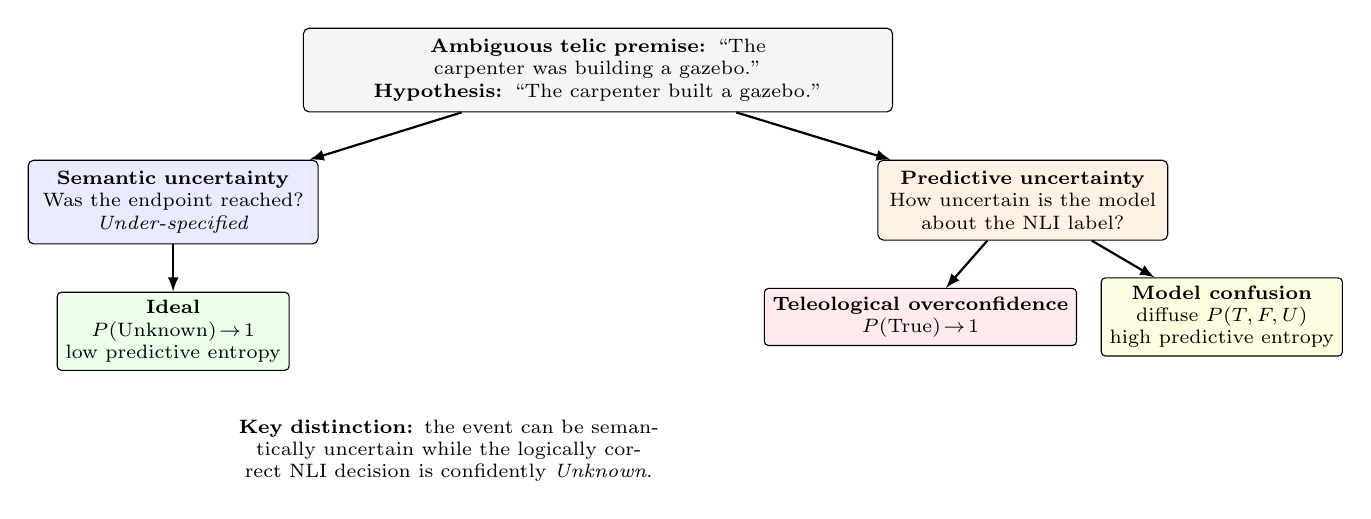
\begin{tikzpicture}[font=\scriptsize, >=latex, node distance=2mm]
\tikzset{box/.style={draw, rounded corners=2pt, align=center, inner sep=4pt, minimum height=8mm},arrow/.style={->, thick},small/.style={draw, rounded corners=1.5pt, align=center, inner sep=3pt, minimum width=25mm}}
\node[box, fill=gray!8, text width=72mm] (premise) {\textbf{Ambiguous telic premise:} ``The carpenter was building a gazebo.''\\\textbf{Hypothesis:} ``The carpenter built a gazebo.''};
\node[box, fill=blue!8, text width=34mm, below left=6mm and -2mm of premise] (world) {\textbf{Semantic uncertainty}\\Was the endpoint reached?\\\emph{Under-specified}};
\node[box, fill=orange!10, text width=34mm, below right=6mm and -2mm of premise] (model) {\textbf{Predictive uncertainty}\\How uncertain is the model\\about the NLI label?};
\draw[arrow] (premise) -- (world); \draw[arrow] (premise) -- (model);
\node[small, fill=green!8, below=6mm of world] (ideal) {\textbf{Ideal}\\$P(\mathrm{Unknown})\!\rightarrow\!1$\\low predictive entropy};
\node[small, fill=red!8, below=6mm of model, xshift=-13mm] (teleo) {\textbf{Teleological overconfidence}\\$P(\mathrm{True})\!\rightarrow\!1$};
\node[small, fill=yellow!12, right=3mm of teleo] (confused) {\textbf{Model confusion}\\diffuse $P(T,F,U)$\\high predictive entropy};
\draw[arrow] (world) -- (ideal); \draw[arrow] (model) -- (teleo); \draw[arrow] (model) -- (confused);
\node[align=center, below=5mm of ideal, xshift=35mm, text width=75mm] {\textbf{Key distinction:} the event can be semantically uncertain while the logically correct NLI decision is confidently \emph{Unknown}.};
\end{tikzpicture}
}
\caption{The central distinction. Group C contains event-level under-specification but has a determinate NLI target. Correct semantic uncertainty is therefore not equivalent to high predictive entropy.}
\label{fig:concept}
\end{figure}

This distinction connects aspectual inference to confidence calibration \citep{guo-etal-2017-calibration,desai-durrett-2020-calibration,jiang-etal-2021-calibration}, confidence elicitation in instruction-tuned LLMs \citep{tian-etal-2023-calibration,xiong-etal-2024-uncertainty}, semantic uncertainty \citep{farquhar-etal-2024-semantic}, uncertainty ranking \citep{huang-etal-2024-rankcalibration}, prompt-sensitive calibration \citep{cox-etal-2025-mapping}, and selective decision making \citep{cole-etal-2023-ambiguous,geifman-el-yaniv-2019-selectivenet,wang-etal-2025-sconu}. It also creates a clean black-box setting: every evaluated endpoint can be asked for a three-way probability report even when provider-specific logits are unavailable or incomparable.

Our objective is not to rerun the earlier benchmark with newer model aliases. Instead, we use its controlled semantics as a laboratory for a distinct reliability question: \emph{when completion is not warranted, can uncertainty expose the failure and support a safer decision rule?} We deliberately evaluate calibration and discrimination separately. A confidence score can be numerically calibrated yet poor at ranking failures; conversely, a useful ranking signal can be miscalibrated in absolute probability. Both properties matter for selective control.

\paragraph{Contributions.} This study makes three planned contributions. First, it formalizes the distinction between event-level semantic uncertainty and model-level predictive uncertainty for imperfective inference and introduces targeted descriptive diagnostics for that distinction. Second, it evaluates two provider-agnostic black-box uncertainty families---structured verbal label probabilities and repeated-sampling disagreement---with paired semantic and prompt-robustness analyses across five API model families. Third, it evaluates uncertainty-aware abstention and selective rechecking using risk--coverage behavior, teleological bias, atelic retention, and operational cost. The design, hypotheses, thresholds, model panel, prompt conditions, and statistical protocol are frozen before examining main-study results.

\section{Background and Related Work}
\subsection{Aspect, Telicity, and Imperfective Inference}
Lexical aspect distinguishes homogeneous activities from goal-bounded accomplishments \citep{vendler-1957-verbs}. For an atelic activity, a non-trivial subinterval can support the occurrence claim; for a telic accomplishment, participation in the process need not imply culmination. The progressive therefore interacts differently with these classes. This is precisely the distinction that makes ``was running'' compatible with ``ran'' while ``was building a house'' does not by itself entail ``built a house.''

Computational work on aspect has shown that representational access to aspectual information does not guarantee robust use of that information at inference time \citep{ma-2024-lexical}. More broadly, diagnostic studies find that language models can arrive at correct answers through shallow heuristics and can underweight negation or other compositional cues \citep{ettinger-2020-bert,kassner-schutze-2020-negated}. ImperfectiveNLI sharpens these concerns by holding lexical material largely constant while manipulating telicity and contextual cancellation \citep{ma-miyao-2026-imperfective}.

The earlier ImperfectiveNLI study evaluated several prompt styles and open-weight models, identifying high completion bias for ambiguous accomplishments and a trade-off in which interventions that suppress telic completion can also damage valid atelic entailments. Our work treats that trade-off as motivation for a different mechanism: rather than globally making a model more skeptical, use uncertainty to decide when skepticism or verification is needed.

\subsection{Confidence, Calibration, and Black-Box Uncertainty}
A probabilistic predictor is calibrated when events assigned a given confidence level are correct at approximately that frequency \citep{guo-etal-2017-calibration}. Language-model calibration is challenging because generated outputs are structured, post-training changes behavior, and API access may hide token-level likelihoods. Prior work nevertheless shows that elicited verbal probabilities can contain useful confidence information \citep{tian-etal-2023-calibration,xiong-etal-2024-uncertainty}, although these self-reports are not guaranteed to be faithful internal probabilities.

Uncertainty over natural-language outputs also depends on what counts as the same answer. Semantic entropy groups generations by meaning rather than treating every string as distinct \citep{farquhar-etal-2024-semantic}. For our three-class NLI setting, semantic equivalence is simpler: each generation is reduced to one of three explicit semantic decisions. Repeated sampling therefore yields a directly interpretable empirical distribution over \{True, False, Unknown\}. We use variation ratio and normalized label entropy as black-box disagreement signals.

Calibration and \emph{ranking} must be separated. Rank-calibration work emphasizes that a useful uncertainty score should order low-quality outputs above high-quality ones in uncertainty even when the score's numeric range differs from another estimator \citep{huang-etal-2024-rankcalibration}. Accordingly, we report proper scoring/calibration measures and error-detection AUROC/AUPRC rather than treating one number as a complete characterization of uncertainty quality.

\subsection{Prompt Sensitivity as an Uncertainty Confound}
Prompt sensitivity is particularly important for confidence experiments. Semantically similar prompts can change an LLM's output distribution and thereby change apparent uncertainty \citep{cox-etal-2025-mapping}. If a paper reports only one prompt, a confidence estimate may partly describe wording sensitivity rather than uncertainty about the task itself. We therefore predeclare one neutral prompt as the primary scientific condition and reserve two semantically motivated interventions---strict logic and definition-aware aspect---for a fixed robustness subset. A label-order reversal provides a separate formatting/order audit. This design prevents choosing whichever prompt looks best after observing benchmark results.

\subsection{Selective Prediction and Verification}
Selective prediction allows a model to abstain or defer rather than force an answer on every input \citep{geifman-el-yaniv-2019-selectivenet}. Recent LLM work similarly studies selective answering and uncertainty-aware guarantees \citep{cole-etal-2023-ambiguous,wang-etal-2025-sconu}. We adopt the operational question relevant to black-box APIs: if uncertainty is high, should a system defer the answer or route it through a more aspect-sensitive verification instruction? A useful uncertainty signal should lower risk as coverage decreases, and a useful verifier should reduce completion bias without simply rejecting all progressive entailments.

\section{Conceptual Framework}
\subsection{Two Levels of Uncertainty}
Let $x=(p,h)$ denote a premise--hypothesis pair and $Y\in\{T,F,U\}$ its NLI label. For Group C, the proposition that the event culminated is not settled by the text. Call this latent event state $Z$. The semantic situation can therefore be under-specified with respect to $Z$ while still fixing $Y=U$. This separation matters because predictive entropy
\begin{equation}
H(\hat{P}(Y\mid x))=-\sum_{y\in\{T,F,U\}}\hat{p}_y\log \hat{p}_y
\end{equation}
can be high for two different reasons: a model may recognize that the world outcome is not entailed, or it may simply be unsure which NLI rule applies. In our task, successful recognition should concentrate probability on $U$; generic confusion may disperse mass across all labels.

This motivates three behavioral states for Group C. \emph{Semantic recognition} corresponds to large $p_U$. \emph{Teleological overconfidence} corresponds to large $p_T$, because the model promotes an ongoing goal-directed process to an attained endpoint. \emph{Predictive confusion} corresponds to diffuse probability mass. These states can have very different reliability implications despite similar entropy values.

\subsection{The Paired Update Test}
ImperfectiveNLI contains a structure that is especially valuable for uncertainty analysis. Telic pair $A_i\leftrightarrow C_i$ shares the verb and hypothesis but removes the explicit cancellation clause: the correct target changes from \textsc{False} to \textsc{Unknown}. Atelic pair $B_i\leftrightarrow D_i$ similarly removes an interruption clause, yet both labels remain \textsc{True}. Figure~\ref{fig:pairwise} summarizes these controlled updates.

\begin{figure}[t]
\centering
\resizebox{\columnwidth}{!}{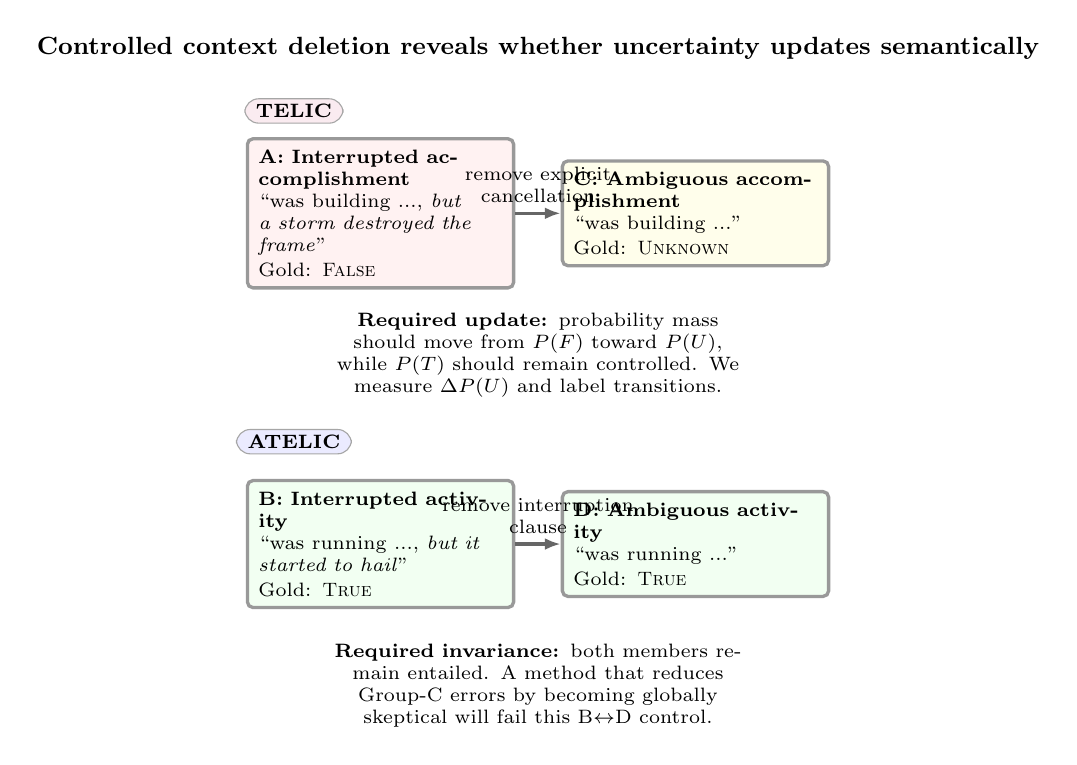
\begin{tikzpicture}[font=\scriptsize,>=Latex]
\tikzset{
  ex/.style={draw=black!40,rounded corners=2pt,very thick,align=left,text width=31mm,inner sep=4pt},
  lab/.style={draw=black!35,rounded corners=5pt,inner xsep=4pt,inner ysep=2pt,font=\scriptsize\bfseries},
  arr/.style={-{Latex[length=2mm]},very thick,draw=black!60}
}

\node[font=\small\bfseries] at (0,3mm) {Controlled context deletion reveals whether uncertainty updates semantically};

% Telic pair
\node[lab,fill=purple!8] at (-31mm,-5mm) {TELIC};
\node[ex,fill=red!5] (A) at (-20mm,-18mm) {
  \textbf{A: Interrupted accomplishment}\\
  ``was building ..., \emph{but a storm destroyed the frame}''\\[1pt]
  Gold: \textsc{False}
};
\node[ex,fill=yellow!8] (C) at (20mm,-18mm) {
  \textbf{C: Ambiguous accomplishment}\\
  ``was building ...''\\[1pt]
  Gold: \textsc{Unknown}
};
\draw[arr] (A.east) -- node[above,align=center]{remove explicit\\cancellation} (C.west);
\node[align=center,text width=68mm] at (0,-36mm) {
  \textbf{Required update:} probability mass should move from $P(F)$ toward $P(U)$,\\
  while $P(T)$ should remain controlled. We measure $\Delta P(U)$ and label transitions.
};

% Atelic pair
\node[lab,fill=blue!8] at (-31mm,-47mm) {ATELIC};
\node[ex,fill=green!5] (B) at (-20mm,-60mm) {
  \textbf{B: Interrupted activity}\\
  ``was running ..., \emph{but it started to hail}''\\[1pt]
  Gold: \textsc{True}
};
\node[ex,fill=green!5] (D) at (20mm,-60mm) {
  \textbf{D: Ambiguous activity}\\
  ``was running ...''\\[1pt]
  Gold: \textsc{True}
};
\draw[arr] (B.east) -- node[above,align=center]{remove interruption\\clause} (D.west);
\node[align=center,text width=68mm] at (0,-78mm) {
  \textbf{Required invariance:} both members remain entailed. A method that reduces\\
  Group-C errors by becoming globally skeptical will fail this B$\leftrightarrow$D control.
};
\end{tikzpicture}
}
\caption{Paired semantic test. A robust model should update from contradiction to uncertainty for telic A$\rightarrow$C while preserving entailment for atelic B$\rightarrow$D.}
\label{fig:pairwise}
\end{figure}

This paired design asks a stronger question than independent group accuracy. For A$\rightarrow$C, does probability mass move from $F$ toward $U$ when cancellation evidence disappears, while avoiding a spurious rise in $T$? For B$\rightarrow$D, does removal of the interruption leave the correct entailment stable? A system that merely learns ``progressive means incomplete'' may improve Group C while failing the atelic control.

\section{Task and Data}
We reuse ImperfectiveNLI from \citet{ma-miyao-2026-imperfective}. The benchmark contains 400 English NLI examples built from 100 telic and 100 atelic verbs. It crosses verb telicity with interrupted versus ambiguous context, producing the four conditions in Table~\ref{tab:groups}. The 100 telic verbs are further grouped into Change of State, Creation, Consumption, and Motion to Goal classes, supporting fine-grained analysis of where completion priors are strongest.

\begin{table}[t]
\centering
\small
\begin{tabular}{@{}llll@{}}
\toprule
Group & Event type & Context & Gold \\
\midrule
A & Telic accomplishment & Interrupted & False \\
B & Atelic activity & Interrupted & True \\
C & Telic accomplishment & Ambiguous & Unknown \\
D & Atelic activity & Ambiguous & True \\
\bottomrule
\end{tabular}
\caption{The four controlled ImperfectiveNLI conditions. Group C is the primary semantic-under-specification probe; Group D is the anti-over-skepticism control.}
\label{tab:groups}
\end{table}

\paragraph{Artifact integrity.} We treat the benchmark as an external research artifact rather than project-owned data. The repository records the upstream repository, path, Git blob identifier, expected file size, and reported CC BY-NC 4.0 license. A downloader retrieves the exact upstream JSON and verifies its Git blob hash. A separate validator checks 400 unique canonical IDs, 100 examples per group, group labels, mandatory fields, and all A$\leftrightarrow$C / B$\leftrightarrow$D lexical pairings before any API calls. The local file's SHA-256 is then stored in each frozen run manifest. This prevents silent benchmark drift.

\section{Research Questions and Predeclared Hypotheses}
\paragraph{RQ1: Uncertainty Recognition.} \emph{Do frontier API LLMs correctly recognize semantic uncertainty in imperfective telic events, and are their confidence distributions calibrated across Groups A--D?} The primary Group-C target is high $P(\textsc{Unknown})$, not merely high entropy. We predeclare that a model exhibiting genuine recognition should have positive Ambiguity Discrimination Gap (defined below), while high-confidence Group-C \textsc{True} predictions indicate teleological overconfidence.

\paragraph{RQ2: Uncertainty Faithfulness.} \emph{Which black-box uncertainty signals---verbalized label probabilities or repeated-sampling disagreement---best identify aspectual errors, teleological completion bias, and overconfidence?} We compare absolute calibration, proper scoring, error ranking, paired probability updates, semantic subclasses, and fixed prompt/order sensitivity. The main hypothesis is deliberately modest: at least one black-box signal should rank errors better than random ordering if the endpoint exposes useful uncertainty.

\paragraph{RQ3: Uncertainty-Aware Control.} \emph{Can selective prediction or selective rechecking reduce teleological completion errors at useful coverage and API cost without degrading valid atelic entailments?} We test whether risk and TBR fall as increasingly uncertain cases are deferred, while Group-D correctness and coverage remain high. We compare the base neutral model, blanket aspect-sensitive verification, and selective verification of only uncertain cases.

\section{Experimental Design}
\subsection{API Model Panel}
We predeclare five model families through a common OpenAI-compatible gateway: \texttt{gpt-5.6-sol}, \texttt{claude-sonnet-5}, \texttt{deepseek-v4-pro}, \texttt{qwen3.8-max}, and \texttt{gemini-3.7-flash}. These are gateway routing identifiers, not claims about immutable vendor-direct checkpoints. Immediately before the frozen run, the artifact queries the live gateway catalog and stores the catalog snapshot. Every response records both the requested and returned identifier, timestamp, decoding settings, request identifier when available, latency, and token usage. Scientific claims in this paper therefore refer to the evaluated gateway routes at the recorded execution time rather than immutable provider checkpoints.

\begin{table}[t]
\centering
\small
\input{generated/model_panel.tex}
\end{table}

No large local model is required. This is intentional: the primary contribution concerns black-box uncertainty signals obtainable under realistic API access constraints, while the gateway-routing limitation is treated explicitly as a threat to validity.

\subsection{Neutral Primary Prompt}
The primary prompt asks the model to perform three-way NLI using only the premise and ordinary word meanings, explicitly disallowing unstated facts but \emph{not} teaching the telic/atelic rule. Providing the relevant linguistic rule in the primary system prompt would confound uncertainty recognition with instruction following. We therefore reserve strict-logic and definition-aware instructions for robustness experiments.

Every deterministic response must be a JSON object containing a label in \{True, False, Unknown\}, a probability distribution $(p_T,p_F,p_U)$, and a one-sentence rationale. The parser checks finite probabilities, range constraints, normalization, and agreement between the stated label and maximum-probability class. Raw responses are retained for auditability. Small rounding deviations are normalized but recorded; label/argmax disagreement is an audit failure rather than silently repaired.

\subsection{Repeated-Sampling Uncertainty}
For RQ2 we draw $K=5$ stochastic generations per item at temperature 0.7 using the same neutral task framing. For sample labels $y_1,\ldots,y_K$, the variation ratio is
\begin{equation}
U_{\mathrm{VR}}=1-\frac{\max_y \sum_{k=1}^{K}\mathbf{1}[y_k=y]}{K},
\end{equation}
and normalized label entropy is the entropy of the empirical three-class sample distribution divided by $\log 3$. Sampling artifacts are audited for exactly $K$ valid records and repeat indices per item; incomplete cases are not quietly treated as low disagreement.

\subsection{Prompt and Label-Order Robustness}
Prompt sensitivity is evaluated on a fixed seed-42, A/B/C/D-balanced subset of 120 examples. Besides the neutral primary instruction, we test (i) a strict-logic prompt that prohibits typicality-based endpoint assumptions and (ii) a definition-aware prompt that explicitly states the aspectual distinction. A separate run reverses output label order from \{True, False, Unknown\} to \{Unknown, False, True\}. These conditions are fixed before results and are not used to select the primary prompt.

For each matched item we report label flip rate, change in correctness, probability shifts, and Jensen--Shannon divergence between the two three-way distributions. This robustness layer directly tests whether a claimed uncertainty effect survives benign changes to task wording or output order \citep{cox-etal-2025-mapping}.

\subsection{Verifier Cache for RQ3}
The RQ3 verifier is an independent aspect-sensitive NLI instruction that first distinguishes telic from atelic events and then applies the corresponding inference rule. It does not receive the base model's answer. For experimental efficiency and clean counterfactual evaluation, we cache one verifier prediction for every model--item pair. We can then simulate all predeclared selective-recheck thresholds without issuing result-dependent API calls. The blanket-verifier condition is a control: if it reduces Group-C bias but harms Group D, selective routing can be evaluated against that trade-off.

\begin{figure}[t]
\centering
\resizebox{\columnwidth}{!}{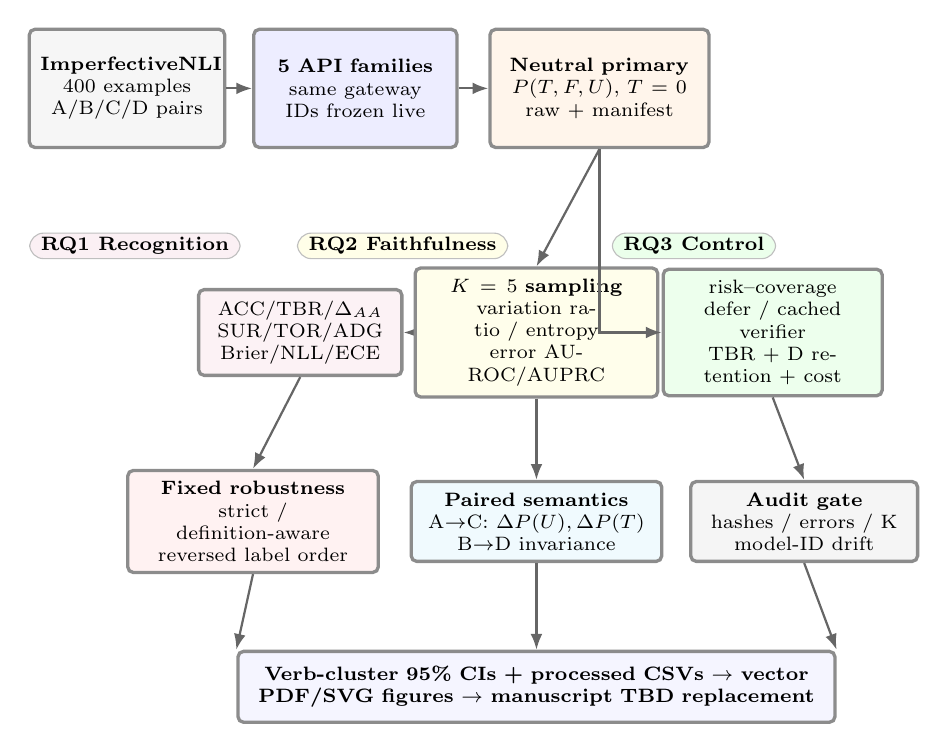
\begin{tikzpicture}[font=\scriptsize,>=Latex]
\tikzset{
  box/.style={draw=black!45,rounded corners=2pt,very thick,align=center,inner sep=4pt},
  arr/.style={-{Latex[length=2mm]},thick,draw=black!60},
  tag/.style={draw=black!25,rounded corners=5pt,inner xsep=4pt,inner ysep=1.5pt,font=\scriptsize\bfseries}
}

\node[box,fill=gray!7,text width=22mm,minimum height=15mm] (data) at (0,0) {
  \textbf{ImperfectiveNLI}\\400 examples\\A/B/C/D pairs
};
\node[box,fill=blue!7,text width=23mm,minimum height=15mm] (models) at (29mm,0) {
  \textbf{5 API families}\\same gateway\\IDs frozen live
};
\node[box,fill=orange!8,text width=25mm,minimum height=15mm] (primary) at (60mm,0) {
  \textbf{Neutral primary}\\$P(T,F,U)$, $T=0$\\raw + manifest
};
\draw[arr] (data) -- (models);
\draw[arr] (models) -- (primary);

\node[tag,fill=purple!6] at (1mm,-20mm) {RQ1 Recognition};
\node[box,fill=purple!5,text width=23mm] (rq1) at (22mm,-31mm) {
  ACC/TBR/$\Delta_{AA}$\\SUR/TOR/ADG\\Brier/NLL/ECE
};
\draw[arr] (primary.south) |- (rq1.east);

\node[tag,fill=yellow!9] at (35mm,-20mm) {RQ2 Faithfulness};
\node[box,fill=yellow!8,text width=28mm] (sample) at (52mm,-31mm) {
  \textbf{$K=5$ sampling}\\variation ratio / entropy\\error AUROC/AUPRC
};
\draw[arr] (primary.south) -- (sample.north);

\node[tag,fill=green!8] at (72mm,-20mm) {RQ3 Control};
\node[box,fill=green!7,text width=25mm] (control) at (82mm,-31mm) {
  risk--coverage\\defer / cached verifier\\TBR + D retention + cost
};
\draw[arr] (primary.south) |- (control.west);

\node[box,fill=red!5,text width=29mm] (robust) at (16mm,-55mm) {
  \textbf{Fixed robustness}\\strict / definition-aware\\reversed label order
};
\node[box,fill=cyan!6,text width=29mm] (paired) at (52mm,-55mm) {
  \textbf{Paired semantics}\\A$\rightarrow$C: $\Delta P(U),\Delta P(T)$\\B$\rightarrow$D invariance
};
\node[box,fill=gray!8,text width=26mm] (audit) at (86mm,-55mm) {
  \textbf{Audit gate}\\hashes / errors / K\\model-ID drift
};
\draw[arr] (rq1.south) -- (robust.north);
\draw[arr] (sample.south) -- (paired.north);
\draw[arr] (control.south) -- (audit.north);

\node[box,fill=blue!4,text width=73mm,minimum height=9mm] (outputs) at (52mm,-76mm) {
  \textbf{Verb-cluster 95\% CIs + processed CSVs $\rightarrow$ vector PDF/SVG figures $\rightarrow$ manuscript TBD replacement}
};
\draw[arr] (robust.south) -- (outputs.north west);
\draw[arr] (paired.south) -- (outputs.north);
\draw[arr] (audit.south) -- (outputs.north east);
\end{tikzpicture}
}
\caption{Black-box evaluation pipeline. Raw API records, manifests, and audit flags are retained before any aggregate result is produced.}
\label{fig:pipeline}
\end{figure}

\subsection{Experiment Matrix and Call Budget}
Table~\ref{tab:matrix} summarizes the frozen main-study budget before retries and smoke testing. The neutral deterministic run contains 2,000 calls and repeated sampling contributes 10,000. The two prompt interventions and label-order audit each use 120 examples per model (1,800 calls total). The full verifier cache contributes 2,000 more. Thus the main study contains 15,800 calls before retries; the 20-example-per-model smoke test adds 100 calls. Actual monetary cost is reported from gateway usage metadata where available rather than estimated from a potentially stale public price table.

\begin{table}[t]
\centering
\small
\begin{tabular}{@{}lrrr@{}}
\toprule
Condition & Items/model & Repeats & Calls \\
\midrule
Neutral deterministic & 400 & 1 & 2,000 \\
Neutral sampling & 400 & 5 & 10,000 \\
Strict robustness & 120 & 1 & 600 \\
Definition robustness & 120 & 1 & 600 \\
Label-order audit & 120 & 1 & 600 \\
Verifier cache & 400 & 1 & 2,000 \\
\midrule
Total & -- & -- & 15,800 \\
\bottomrule
\end{tabular}
\caption{Predeclared main-study API call budget across five models, excluding retries and the 100-call smoke test.}
\label{tab:matrix}
\end{table}

\section{Metrics and Statistical Protocol}
\subsection{Benchmark Metrics}
We retain the original group-wise accuracies, Teleological Bias Rate on Group C, and Aspectual Awareness Gap \citep{ma-miyao-2026-imperfective}. With predictions $\hat y_i$,
\begin{equation}
\mathrm{TBR}_{C}=\frac{1}{|C|}\sum_{i\in C}\mathbf{1}[\hat y_i=T],
\end{equation}
and $\Delta_{AA}=\mathrm{ACC}_D-\mathrm{TBR}_{C}$. TBR isolates the specific false-completion behavior rather than treating all Group-C errors as equivalent.

\subsection{Uncertainty-Specific Diagnostics}
We introduce three descriptive paper-specific measures:
\begin{align}
\mathrm{SUR} &= \mathbb{E}[p_U \mid C],\\
\mathrm{TOR}_{\tau} &= \Pr(p_T\ge \tau \mid C),\\
\mathrm{ADG} &= \mathbb{E}[p_U\mid C]-\mathbb{E}[p_U\mid A,B,D].
\end{align}
SUR (Semantic Uncertainty Recognition) measures probability assigned to the correct uncertainty label. TOR (Teleological Overconfidence Rate) measures high-confidence completion assertions in the ambiguous telic condition; we predeclare $\tau=.80$ for compact reporting and also retain threshold behavior. ADG measures whether uncertainty is selective rather than globally inflated. These are proposed descriptive metrics for this study, not established community standards.

\subsection{Calibration, Scoring, and Failure Detection}
Absolute probability quality is measured with multiclass Brier score, negative log-likelihood, top-label expected calibration error (15 equal-width bins), and one-vs-rest classwise ECE. We emphasize Unknown-class calibration because aggregate ECE can hide systematic behavior on the scientifically critical Group C.

Discrimination is evaluated separately. For each uncertainty score---$1-\max_y p_y$, normalized predictive entropy, sampling variation ratio, and sampling label entropy---we treat incorrect predictions as the positive class and report error-detection AUROC and AUPRC. We report both all-example and Group-C-only rankings. This avoids claiming that a well-calibrated score is necessarily useful for finding failures. Reliability diagrams and risk-ranking analyses are generated from processed artifacts, not manually transcribed values.

\subsection{Paired Context-Update Metrics}
For each A$\rightarrow$C pair we measure $\Delta p_U=p_U(C)-p_U(A)$ and $\Delta p_T=p_T(C)-p_T(A)$, together with the full label-transition matrix. Positive $\Delta p_U$ is expected when explicit cancellation is removed; an uncontrolled increase in $p_T$ reveals a completion prior. For B$\rightarrow$D we test stability of the correct True decision. Telic A/C shifts are additionally reported by semantic subclass. This analysis uses the benchmark's controlled pairing rather than treating its 400 rows as independent observations.

\subsection{Selective Risk}
For uncertainty score $u_i$, examples are ordered from least to most uncertain. We report selective risk across coverage, empirical AURC, and empirical excess AURC above an oracle ordering. Because $K=5$ sampling scores are discrete and create many ties, AURC uses the expected cumulative error under a uniformly random ordering within each tied score block, making the estimate invariant to row order. Fixed-coverage operating points are threshold-realizable: if a requested coverage cuts through a tied block, the full block is retained and the achieved coverage is reported. Coverage at target risks of 10\% and 5\% is likewise computed only at attainable score thresholds.

A generic abstention metric can hide the exact failure of interest, so every RQ3 operating point also reports Group-C TBR, Group-C coverage, Group-D coverage, and Group-D retained accuracy. A method cannot be credited for ``solving'' completion bias merely by disproportionately dropping progressive examples.

\subsection{Selective Recheck Policies}
We compare three policies: (1) base neutral predictions for all items; (2) blanket verifier predictions for all items; and (3) selective recheck, which replaces the base prediction with the cached verifier only when base uncertainty exceeds a predeclared threshold. The full threshold sweep is primary evidence. For one compact manuscript table we predeclare $1-\max p\ge0.20$ as an operating point before observing results; it is not selected post hoc. Reported cost includes recheck call rate, base tokens, incremental verifier tokens, total simulated policy tokens, and incremental-token ratio.

\subsection{Uncertainty Intervals and Multiple Testing}
Because examples are paired by lexical verb, primary uncertainty intervals are obtained through 10,000 verb-cluster bootstrap resamples with 95\% percentile intervals. We avoid treating the 400 templated rows as independent IID evidence. Families of multi-model hypothesis tests use Holm correction. If any threshold is optimized rather than reported as a predeclared sweep, it is selected on a verb-disjoint calibration split and evaluated on held-out verbs. Post-hoc exploratory analyses are labeled as such.

\subsection{Sanity Baselines}
We include simple analytical baselines---always True, always Unknown, and a uniform three-way probability distribution---to make new metrics interpretable. For example, uniform output has high predictive entropy but should not be mistaken for successful semantic uncertainty recognition. These baselines are negative controls for metric interpretation, not competing LLM systems.

\section{Reproducibility and Audit Gate}
Each frozen run has a stable run identifier and its own output directory. The manifest records dataset SHA-256, exact selected example IDs, model/configuration hashes, prompt hash, label order, decoding settings, maximum output tokens, git commit, Python version, and platform. Each response records requested and returned model IDs, exact message hash, requested seed, timestamp, latency, provider usage metadata when supplied, raw response, parsed prediction, and parsing diagnostics.

Before analysis, an automated audit validates each output against its frozen manifest. It checks malformed JSONL, duplicate example--repeat keys, exact ID coverage, repeat-index sets, expected row count, request/parse failures, label/argmax consistency, probability normalization, prompt hash, label order, decoding settings, model-file coverage, and current dataset/config hashes. A failed audit stops downstream analysis. Interrupted runs can resume only when critical manifest fields match; failed request/parse rows can be atomically purged and replaced without introducing duplicate keys.

The raw gateway key is read only from the local environment variable \texttt{ZZZ\_API\_KEY}; it is never stored in Git. Windows and POSIX scripts execute the same smoke gate, paid calls, audits, analyses, vector figures, and generated LaTeX tables. Numerical table cells are produced by code from audited CSVs rather than copied manually into the manuscript.

% Execution-validation record generated from the 2026-09-03 frozen smoke sequence.
% IMPORTANT: this file is an engineering/audit record, NOT main-study empirical evidence.
% It must not be cited as RQ1/RQ2/RQ3 evidence. The manuscript Results section remains TBD
% until all frozen main-study runs pass the manifest-aware audit.

\paragraph{Execution-validation record (2026-09-03; non-evidentiary smoke).}
Immediately before the smoke sequence, repeated gateway-catalogue snapshots exposed all five predeclared routing identifiers---\texttt{gpt-5.6-sol}, \texttt{claude-sonnet-5}, \texttt{deepseek-v4-pro}, \texttt{qwen3.8-max}, and \texttt{gemini-3.7-flash}---within a catalogue of 842 entries. The snapshots had identical catalogue SHA-256 \texttt{904b9ec7a7b04d7e9e709558d58d2cfbffda0ebf9cdc1390b0543a6fd7b7157a}; no API credential was recorded.

The first balanced 20-example-per-model deterministic neutral smoke issued 100 paid completion calls. Request failures were zero for all five routed endpoints. The hard audit nevertheless failed because structured-output parsing failed for 12/20 DeepSeek responses and 6/20 Gemini responses. Claude, GPT, and Qwen each produced 20/20 parse-valid records. Because the smoke audit failed, no smoke metric was promoted into the scientific Results section and the 15,800-call main study remained blocked.

\begin{table}[t]
\centering
\small
\begin{tabular}{@{}lrrrr@{}}
\toprule
Gateway route & V1 valid & V2 valid & V3 valid & V4 valid \\
\midrule
\texttt{gpt-5.6-sol} & 20/20 & 20/20 & 20/20 & 20/20 \\
\texttt{claude-sonnet-5} & 20/20 & 20/20 & 20/20 & 20/20 \\
\texttt{deepseek-v4-pro} & 8/20 & 17/20 & 18/20 & 20/20 \\
\texttt{qwen3.8-max} & 20/20 & 20/20 & 20/20 & 20/20 \\
\texttt{gemini-3.7-flash} & 14/20 & 20/20 & 20/20 & 20/20 \\
\bottomrule
\end{tabular}
\caption{Non-evidentiary smoke-test structured-output validity across compatibility freezes. These counts are execution gates, not RQ results.}
\label{tab:smoke-execution-validation}
\end{table}

\paragraph{Failure-shape diagnosis.}
Inspection of preserved V1 raw responses established completion-budget exhaustion rather than a general semantic-label parser incompatibility. Every failed DeepSeek response had \texttt{finish\_reason=length} and exactly 220 completion tokens. Eleven had empty final \texttt{content} while exposing long \texttt{reasoning\_content}; the remaining response emitted only a JSON prefix before the budget ended. For Gemini, all six failed message bodies were visibly incomplete JSON/code-fence prefixes. Four reported \texttt{finish\_reason=length}; two reported \texttt{finish\_reason=stop} despite still being incomplete.

\paragraph{V2--V3 compatibility checks.}
Before any main-study result existed, \texttt{experiment-ready-v2} changed exactly one execution setting: the maximum completion budget from 220 to 1024 tokens. The complete 15,800-request offline plan was re-frozen and re-audited with zero completion calls. A fresh 100-call V2 smoke then made Gemini fully parse-valid (20/20) and improved DeepSeek from 8/20 to 17/20. The only three remaining DeepSeek failures were \texttt{A\_015}, \texttt{D\_007}, and \texttt{A\_036}; all ended with \texttt{finish\_reason=length}. \texttt{experiment-ready-v3} therefore raised only the completion ceiling from 1024 to 4096 tokens and added a hard completion-budget audit. V3 improved DeepSeek to 18/20, but \texttt{A\_015} and \texttt{D\_007} still exhausted the full 4096-token ceiling and failed parsing. GPT, Claude, Qwen, and Gemini remained 20/20 parse-valid.

\paragraph{V4 final compatibility gate.}
Because repeated ceiling increases did not eliminate DeepSeek reasoning-budget exhaustion and would not by themselves guarantee the intended temperature-controlled repeated-sampling condition, \texttt{experiment-ready-v4} froze a model-specific request override for \texttt{deepseek-v4-pro} that disables gateway thinking mode while keeping the 4096-token ceiling and every scientific setting unchanged. A fresh balanced 100-call V4 smoke passed the manifest-aware run audit for all five routes: each model produced 20/20 valid records, with zero request failures and zero parse failures. The independent completion-budget audit checked all 100 preserved responses and found zero \texttt{finish\_reason=length} rows. A dedicated model-control audit also reported zero override mismatches and zero forbidden DeepSeek reasoning-content violations. The V4 smoke outputs were integrity-sealed with a SHA-256 run manifest. This establishes execution compatibility only; the smoke summary remains quarantined from RQ1/RQ2/RQ3 inference.

The neutral prompt, RQs, hypotheses, model routes, dataset, temperatures, sampling $K$, robustness subsets, thresholds, metrics, and statistical protocol were not changed by the V4 compatibility fix. V1--V4 remain provenance checkpoints; no failed smoke value is promoted into the manuscript Results section.


\section{Results and Analysis}
All empirical values in this section remain \textbf{TBD} until the corresponding raw artifacts exist and the audit gate passes. The table and figure layout is frozen in advance to reduce flexibility in result selection.

\subsection{RQ1: Do Models Recognize Imperfective Uncertainty?}
Table~\ref{tab:rq1} reports the original task metrics together with SUR, TOR@0.80, and calibration after execution. The first analysis asks whether high Group-C accuracy is accompanied by high $p_U$, or whether apparently correct predictions are low-confidence guesses. We then contrast Unknown-class calibration with aggregate calibration and inspect telic semantic subclasses. Companion generated artifacts contain ADG, Brier, NLL, and verb-cluster intervals.

% PRE-RUN PLACEHOLDER. Overwritten only by scripts/make_paper_tables.py after PASS audits.
\begin{table*}[t]
\centering
\scriptsize
\begin{tabular}{@{}lccccccccc@{}}
\toprule
Model & Acc A & Acc B & Acc C & Acc D & TBR$\downarrow$ & $\Delta_{AA}\uparrow$ & SUR$\uparrow$ & TOR$.80\downarrow$ & ECE$\downarrow$ \\
\midrule
\texttt{gpt-5.6-sol} & TBD & TBD & TBD & TBD & TBD & TBD & TBD & TBD & TBD \\
\texttt{claude-sonnet-5} & TBD & TBD & TBD & TBD & TBD & TBD & TBD & TBD & TBD \\
\texttt{deepseek-v4-pro} & TBD & TBD & TBD & TBD & TBD & TBD & TBD & TBD & TBD \\
\texttt{qwen3.8-max} & TBD & TBD & TBD & TBD & TBD & TBD & TBD & TBD & TBD \\
\texttt{gemini-3.7-flash} & TBD & TBD & TBD & TBD & TBD & TBD & TBD & TBD & TBD \\
\bottomrule
\end{tabular}
\caption{RQ1 primary results generated from the audited neutral deterministic run. Brier, NLL, ADG, classwise ECE, and verb-cluster 95\% intervals are emitted in companion artifacts.}
\label{tab:rq1}
\end{table*}


\subsection{RQ2: Which Uncertainty Signal Is Faithful?}
We compare verbalized uncertainty and sampling disagreement for error ranking, then examine whether the signals remain stable under prompt and label-order changes. The paired A$\rightarrow$C analysis asks whether probability changes in the semantically appropriate direction when cancellation evidence is removed; B$\rightarrow$D serves as the control. We report label-flip rate and mean Jensen--Shannon divergence for each robustness condition rather than selecting representative examples.

% PRE-RUN PLACEHOLDER. Overwritten only by scripts/make_paper_tables.py after PASS audits.
\begin{table}[t]
\centering
\small
\begin{tabular}{@{}lccc@{}}
\toprule
Signal & Error AUROC & Error AUPRC & E-AURC \\
\midrule
$1-\max p$ & TBD & TBD & TBD \\
Predictive entropy & TBD & TBD & TBD \\
Sampling variation & TBD & TBD & TBD \\
Sampling entropy & TBD & TBD & TBD \\
\bottomrule
\end{tabular}
\caption{RQ2 uncertainty-faithfulness placeholder. The post-run generator expands this into per-model rows for all four predeclared signals; no best-signal selection is performed.}
\label{tab:rq2}
\end{table}


\subsection{RQ3: Can Uncertainty Control Risk?}
The primary visualization is the risk--coverage curve for each black-box signal, accompanied by TBR and Group-D retention at matched attainable coverage. We then compare base, blanket-verifier, and selective-recheck policies. The key test is not whether an aspect-aware instruction can lower Group-C errors in isolation, but whether uncertainty can route that intervention selectively enough to preserve valid atelic entailments and reduce API/token cost.

% PRE-RUN PLACEHOLDER. Overwritten only by scripts/make_paper_tables.py after PASS audits.
\begin{table}[t]
\centering
\small
\begin{tabular}{@{}lccccc@{}}
\toprule
Policy & Risk$\downarrow$ & TBR$\downarrow$ & D Acc$\uparrow$ & Recheck & Added tokens \\
\midrule
Base neutral & TBD & TBD & TBD & 0\% & 0 \\
Blanket verifier & TBD & TBD & TBD & 100\% & TBD \\
Selective recheck & TBD & TBD & TBD & TBD & TBD \\
\bottomrule
\end{tabular}
\caption{RQ3 policy placeholder. The generated table uses the predeclared selective operating point from \texttt{configs/experiment.yaml}; full sweeps are retained in processed artifacts.}
\label{tab:rq3}
\end{table}


\begin{figure}[t]
\centering
\IfFileExists{../results/figures/rq1_group_c_uncertainty.pdf}{%
  \includegraphics[width=\columnwidth]{../results/figures/rq1_group_c_uncertainty.pdf}%
}{%
  \resizebox{\columnwidth}{!}{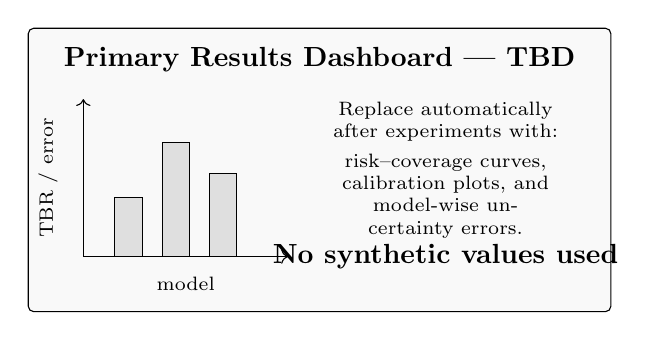
\begin{tikzpicture}[font=\scriptsize]
\draw[rounded corners=2pt, fill=gray!5] (0,0) rectangle (7.4,3.6);
\node[font=\bfseries] at (3.7,3.2) {Primary Results Dashboard --- TBD};
\draw[->] (0.7,0.7) -- (0.7,2.7); \draw[->] (0.7,0.7) -- (3.3,0.7);
\node[rotate=90] at (0.25,1.7) {TBR / error}; \node at (2.0,0.35) {model};
\draw[fill=gray!25] (1.1,0.7) rectangle (1.45,1.45); \draw[fill=gray!25] (1.7,0.7) rectangle (2.05,2.15); \draw[fill=gray!25] (2.3,0.7) rectangle (2.65,1.75);
\node[align=center, text width=32mm] at (5.3,1.8) {Replace automatically after experiments with:\\[1mm]risk--coverage curves,\\calibration plots, and\\model-wise uncertainty errors.};
\node[font=\bfseries] at (5.3,0.7) {No synthetic values used};
\end{tikzpicture}
}%
}
\caption{Primary empirical visualization. Before execution this renders an explicit TBD layout; after audited analysis it is loaded directly from the generated vector result artifact.}
\label{fig:primary-results}
\end{figure}

\subsection{Qualitative Failure Analysis}
Qualitative analysis is prestratified rather than anecdotal. We sample cases by model, group, confidence regime, and telic semantic class, preserving the model's one-sentence rationale. Candidate error codes are endpoint-completion prior, cancellation neglect, over-skepticism, telicity confusion, and probability/label inconsistency. Counts are reported only after a documented coding pass; examples explain aggregate patterns rather than substitute for them.

\section{Safety Relevance and Scope}
The benchmark measures a linguistic inference failure, not end-to-end system safety. Nevertheless, completion assumptions can matter in systems that consume natural-language state reports. A monitor that maps ``was verifying,'' ``was shutting down,'' ``was patching,'' or ``was repairing'' to a completed state can propagate an unsupported success condition downstream. The reverse failure also matters: a globally skeptical intervention may reject legitimate claims of activity occurrence and degrade utility.

Our safety claim is deliberately narrow. ImperfectiveNLI is a controlled test of whether models respect an event-semantic boundary and whether uncertainty exposes violations of that boundary. Lower TBR does not by itself demonstrate safe deployment. The contribution lies in evaluation and risk quantification, plus a lightweight selective-control experiment that makes the uncertainty signal operational.

\section{Threats to Validity}
\paragraph{Construct validity.} Elicited probabilities are model outputs, not direct measurements of a hidden Bayesian posterior. They can be strategic, instruction-sensitive, rounded, or otherwise unfaithful. Repeated sampling and prompt robustness provide independent behavioral checks but do not eliminate this limitation. Likewise, Group C's \textsc{Unknown} is the benchmark's normative NLI target; it is not an empirical distribution of human beliefs over possible event completions.

\paragraph{Internal validity.} The benchmark is template-controlled, which is valuable for causal contrasts but may introduce lexical regularities. We exploit the paired structure and bootstrap by verb to reduce pseudo-replication. We do not alter labels after observing results. The neutral primary prompt is fixed before the main run to avoid a knowledge-injection confound.

\paragraph{External validity.} The benchmark is English-only and centered on one aspectual phenomenon. Performance may differ in languages with different aspect marking, longer discourse, or domain-specific operational text. Our safety interpretation is therefore a test-case argument rather than a claim of broad deployment reliability.

\paragraph{API and routing validity.} The experiment accesses models through a third-party OpenAI-compatible gateway rather than auditing vendor-direct checkpoints. A gateway may change routing, system layers, sampling behavior, or aliases, and a requested identifier does not prove immutable backend identity. We therefore freeze the live catalog and retain returned identifiers and timestamps. Claims are about the evaluated routed endpoints on the recorded date; exact numerical reproduction may become impossible if those routes disappear.

\paragraph{Statistical conclusion validity.} The 400 rows are not 400 independent lexical concepts. Verb-cluster bootstrap intervals, paired analyses, tie-aware selective risk, and corrected hypothesis families are used to avoid overstating effective sample size or exploiting arbitrary score ordering. Small telic subclasses should be interpreted with correspondingly wider uncertainty.

\section{Ethical and Artifact Considerations}
The study does not require new human-subject data or personally identifiable information. The reused dataset is attributed to its original authors and handled under the license reported in the source release. Project code and third-party data are kept legally distinct rather than silently re-licensing the benchmark under the repository's software license.

The experiment uses API-accessed LLMs and therefore consumes compute and monetary resources. We report call counts, token usage when supplied, and the incremental cost of selective verification. Caching verifier predictions avoids repeatedly paying for the same response during threshold analysis. API keys and other credentials are excluded from version control.

AI assistance may be used for code scaffolding, grammar, and manuscript drafting, but research decisions, reference checks, experimental execution, result interpretation, and final claims remain the responsibility of the authors. Model-generated rationales in the released artifact are short requested explanations, not hidden chain-of-thought and not treated as privileged access to internal reasoning.

\section{Statement of Contributions}
This paper extends the ImperfectiveNLI line of work along a new uncertainty and control axis rather than presenting a model-only replication. It (i) distinguishes event-level semantic under-specification from predictive uncertainty for aspectual inference; (ii) evaluates cross-family black-box verbal and sampling uncertainty; (iii) adds paired semantic-update and prompt-sensitivity diagnostics; and (iv) tests uncertainty-aware abstention and verification under explicit risk, retention, and cost metrics. The earlier dataset, task design, and original teleological-bias metrics are explicitly attributed. New metrics are labeled as paper-specific descriptive diagnostics. Every empirical claim will be traceable to a frozen run manifest and raw API output.

\section{Conclusion}
We introduce \emph{imperfective uncertainty} as a reliability problem: whether an LLM can represent and use uncertainty appropriately when an event's endpoint is not semantically licensed. The imperfective paradox creates a revealing separation between an under-specified world state and a determinate \textsc{Unknown} inference. This makes it possible to distinguish semantic recognition from both teleological overconfidence and generic predictive confusion. Our evaluation combines calibrated confidence, repeated-sampling disagreement, paired semantic updates, prompt robustness, and selective control. The resulting design asks not only whether a model is wrong, but whether its uncertainty makes that failure detectable, rankable, and controllable without sacrificing valid atelic reasoning. Empirical conclusions remain \textbf{TBD} pending the frozen experiment.

\begin{thebibliography}{99}
\bibitem[Ma and Miyao(2026)]{ma-miyao-2026-imperfective} Bolei Ma and Yusuke Miyao. 2026. The Imperfective Paradox in Large Language Models. In \emph{Proceedings of ACL 2026 (Volume 1: Long Papers)}, 15093--15111. Association for Computational Linguistics.
\bibitem[Ma(2024)]{ma-2024-lexical} Bolei Ma. 2024. Evaluating Lexical Aspect with Large Language Models. In \emph{Proceedings of the Workshop on Cognitive Modeling and Computational Linguistics}, 123--131. doi:10.18653/v1/2024.cmcl-1.11.
\bibitem[Jiang et~al.(2021)]{jiang-etal-2021-calibration} Zhengbao Jiang, Jun Araki, Haibo Ding, and Graham Neubig. 2021. How Can We Know When Language Models Know? On the Calibration of Language Models for Question Answering. \emph{TACL}, 9:962--977. doi:10.1162/tacl\_a\_00407.
\bibitem[Tian et~al.(2023)]{tian-etal-2023-calibration} Katherine Tian, Eric Mitchell, Allan Zhou, Archit Sharma, Rafael Rafailov, Huaxiu Yao, Chelsea Finn, and Christopher D. Manning. 2023. Just Ask for Calibration: Strategies for Eliciting Calibrated Confidence Scores from Language Models Fine-Tuned with Human Feedback. In \emph{EMNLP 2023}, 5433--5442. doi:10.18653/v1/2023.emnlp-main.330.
\bibitem[Cole et~al.(2023)]{cole-etal-2023-ambiguous} Jeremy Cole, Michael Zhang, Daniel Gillick, Julian Eisenschlos, Bhuwan Dhingra, and Jacob Eisenstein. 2023. Selectively Answering Ambiguous Questions. In \emph{EMNLP 2023}, 530--543. doi:10.18653/v1/2023.emnlp-main.35.
\bibitem[Xiong et~al.(2024)]{xiong-etal-2024-uncertainty} Miao Xiong, Zhiyuan Hu, Xinyang Lu, Yifei Li, Jie Fu, Junxian He, and Bryan Hooi. 2024. Can LLMs Express Their Uncertainty? An Empirical Evaluation of Confidence Elicitation in LLMs. In \emph{The Twelfth International Conference on Learning Representations}.
\bibitem[Farquhar et~al.(2024)]{farquhar-etal-2024-semantic} Sebastian Farquhar, Jannik Kossen, Lorenz Kuhn, and Yarin Gal. 2024. Detecting Hallucinations in Large Language Models Using Semantic Entropy. \emph{Nature}, 630:625--630. doi:10.1038/s41586-024-07421-0.
\bibitem[Huang et~al.(2024)]{huang-etal-2024-rankcalibration} Xinmeng Huang, Shuo Li, Mengxin Yu, Matteo Sesia, Hamed Hassani, Insup Lee, Osbert Bastani, and Edgar Dobriban. 2024. Uncertainty in Language Models: Assessment through Rank-Calibration. In \emph{EMNLP 2024}, 284--312. doi:10.18653/v1/2024.emnlp-main.18.
\bibitem[Cox et~al.(2025)]{cox-etal-2025-mapping} Kyle Cox, Jiawei Xu, Yikun Han, Rong Xu, Tianhao Li, Chi-Yang Hsu, Tianlong Chen, Walter Gerych, and Ying Ding. 2025. Mapping from Meaning: Addressing the Miscalibration of Prompt-Sensitive Language Models. In \emph{Proceedings of the AAAI Conference on Artificial Intelligence}, 39(22):23696--23703. doi:10.1609/aaai.v39i22.34540.
\bibitem[Wang and Holmes(2025)]{wang-holmes-2025-subjective} Ziyu Wang and Christopher C. Holmes. 2025. On Subjective Uncertainty Quantification and Calibration in Natural Language Generation. In \emph{AISTATS 2025}, PMLR 258:3799--3807.
\bibitem[Wang et~al.(2025)]{wang-etal-2025-sconu} Zhiyuan Wang, Qingni Wang, Yue Zhang, Tianlong Chen, Xiaofeng Zhu, Xiaoshuang Shi, and Kaidi Xu. 2025. SConU: Selective Conformal Uncertainty in Large Language Models. In \emph{ACL 2025 (Volume 1: Long Papers)}, 19052--19075. doi:10.18653/v1/2025.acl-long.934.
\bibitem[Desai and Durrett(2020)]{desai-durrett-2020-calibration} Shrey Desai and Greg Durrett. 2020. Calibration of Pre-trained Transformers. In \emph{EMNLP 2020}, 295--302. doi:10.18653/v1/2020.emnlp-main.21.
\bibitem[Guo et~al.(2017)]{guo-etal-2017-calibration} Chuan Guo, Geoff Pleiss, Yu Sun, and Kilian Q. Weinberger. 2017. On Calibration of Modern Neural Networks. In \emph{ICML 2017}, PMLR 70:1321--1330.
\bibitem[Geifman and El-Yaniv(2019)]{geifman-el-yaniv-2019-selectivenet} Yonatan Geifman and Ran El-Yaniv. 2019. SelectiveNet: A Deep Neural Network with an Integrated Reject Option. In \emph{ICML 2019}, PMLR 97:2151--2159.
\bibitem[Ettinger(2020)]{ettinger-2020-bert} Allyson Ettinger. 2020. What BERT Is Not: Lessons from a New Suite of Psycholinguistic Diagnostics for Language Models. \emph{TACL}, 8:34--48. doi:10.1162/tacl\_a\_00298.
\bibitem[Kassner and Schuetze(2020)]{kassner-schutze-2020-negated} Nora Kassner and Hinrich Schuetze. 2020. Negated and Misprimed Probes for Pretrained Language Models: Birds Can Talk, But Cannot Fly. In \emph{ACL 2020}, 7811--7818. doi:10.18653/v1/2020.acl-main.698.
\bibitem[Vendler(1957)]{vendler-1957-verbs} Zeno Vendler. 1957. Verbs and Times. \emph{The Philosophical Review}, 66(2):143--160.
\bibitem[Dowty(1979)]{dowty-1979-word} David R. Dowty. 1979. \emph{Word Meaning and Montague Grammar}. D. Reidel.
\bibitem[Comrie(1976)]{comrie-1976-aspect} Bernard Comrie. 1976. \emph{Aspect}. Cambridge University Press.
\end{thebibliography}

\end{document}
